\documentclass[11pt, a4paper]{article}

\usepackage{amsmath}
\usepackage{hyperref}
\usepackage{graphicx}
\usepackage{listings}
\usepackage{color}

\author{
  VIVEK SANGWAN\\
  \texttt{12D070033}
  \and
  KUSH MOTWANI\\
  \texttt{12D070018}
  \and
  \textbf{KOTWAL ALANKAR SHASHIKANT}\\
  \texttt{12D070010}
  \and
}
\title{A PCA-Based Strong Gravitational Lens Finder}

\begin{document}
\maketitle
\newpage

\section{Introduction}
Gravitational lensing is one of the most visible implications of Einstein’s General Theory of Relativity. This effect predicts that light is bent by gravitational fields. In particular, if we have a heavy object in directly front of a source of light in our line of sight, this effect causes ring- and arc-like features like those shown below:\\ \\
\centerline{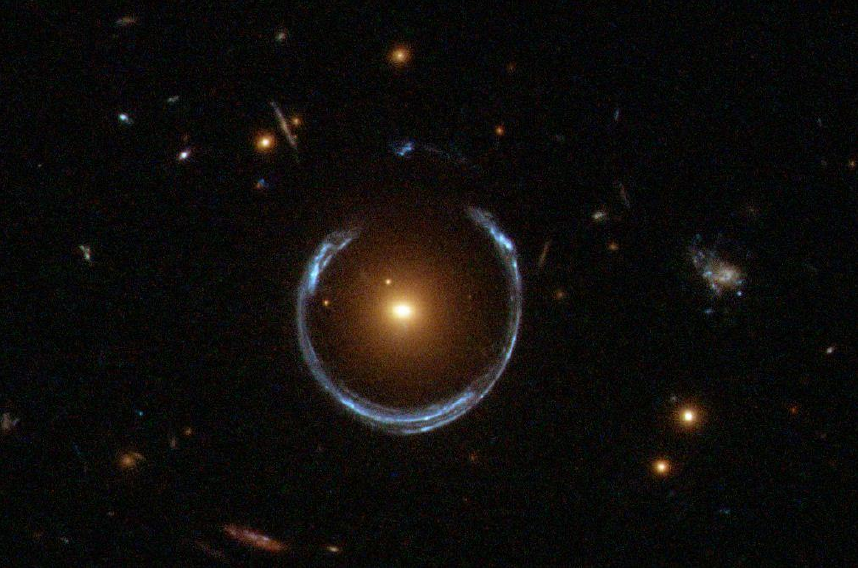
\includegraphics[scale=0.35]{lens_intro.png}}
\\ \\
Our job here is to identify these features without modifying their size and shape. The size and shape of a ring contains vital information about the configuration of the system, especially the mass of the lens. If our method is to be useful for further processing, we must recover the arc as it was in the original image. We exploit PCA and the fact that lenses are rare objects in order to efficiently reconstruct the central galaxy, subtract it from the image and get the arc. A sample output (from this project itself), for instance, would be: \\ \\
\centerline{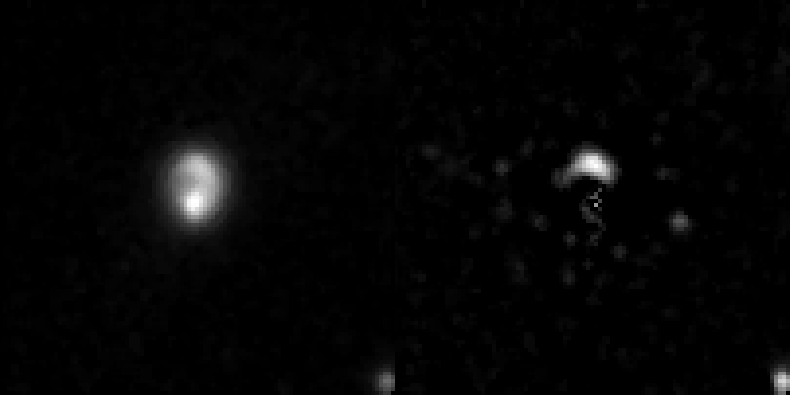
\includegraphics[scale=0.4]{montage.png}}
\\ \\
The left image is the original, and on the right the central source has been subtracted to leave only the ring.

\section{Method}
The method we follow is a slightly modified version of the paper \textit{Joseph, R., Courbin F. et al. 2014, A PCA-based Automated Finder for Galaxy-Scale Strong Lenses}. You can find the paper \href{http://arxiv.org/pdf/1403.1063v1.pdf}{here}.

The fact that the lensing patterns are rare among galaxies in general is used. We construct a PCA basis for aligned galaxy images using the train dataset. In this basis, the galaxies in the frame are represented adequately, and the lensing features, being rare, are under-represented. As a consequence, reconstructing the galaxy image from this basis yields mostly only the bright central core of the object. Subtracting the reconstructed image from the original image is therefore expected to yield the (non-reconstructed) lensing features. Denoising, thresholding and segmentation of the subtracted image can give an image (andhopefully measurements) of the features that further help in lens mass estimation.

We implemented the algorithm in Matlab. Detailed steps are explained in the following section.

\section{Implementation}

\subsection{Iteration 1}

Images were acquired from the simulated KiDS database for gravitational lenses. In the very first trial, all images were taken into consideration and no denoising was applied. A PCA basis was constructed and the first 150 eigenvectors were kept as recommended in the paper. No statistics on the results of the iteration were done since this was the preliminary step. Some primary results obtained and primary observations are as follows:

\begin{itemize}
\item The method works, and the principle is correct. For example, from this iteration, a result is presented below: \\ \\
\centerline{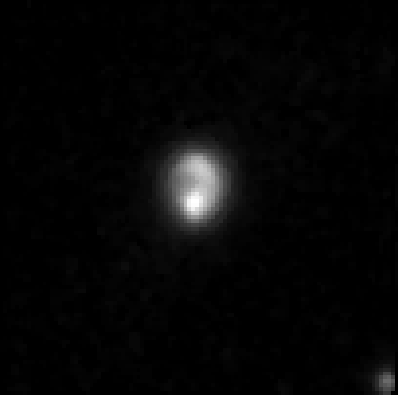
\includegraphics[scale=0.5]{first_object.png} 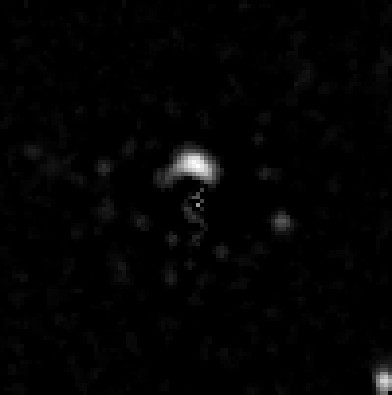
\includegraphics[scale=0.5]{first_ring.png}}
\\ \\ The left image is the original, and on the right the central source has been subtracted to leave only the ring.
\item However, we don't get good reconstructions for most other objects because of a variety of factors. Some of them are instrinsic to the objects we're dealing with, like:
	\begin{itemize}
	\item Size differences: Galaxies come in a variety of sizes as seen from us as a result of both their intrinsic sizes and their distances from us. An example from the database: \\ \\
	\centerline{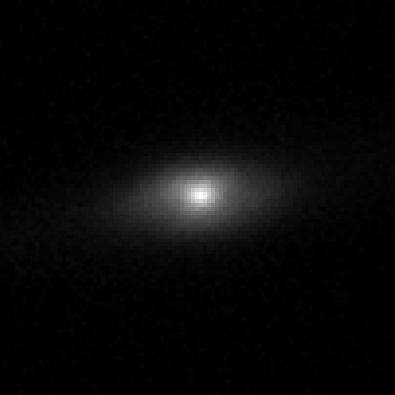
\includegraphics[scale=0.5]{big_galaxy.png}  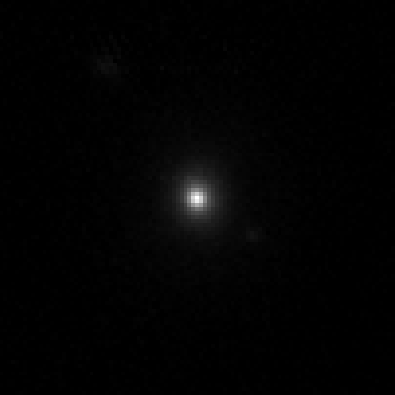
\includegraphics[scale=0.5]{small_galaxy.png}}
	\item Orientation differences: Galaxies are scattered at random orientations. \\ \\
	\centerline{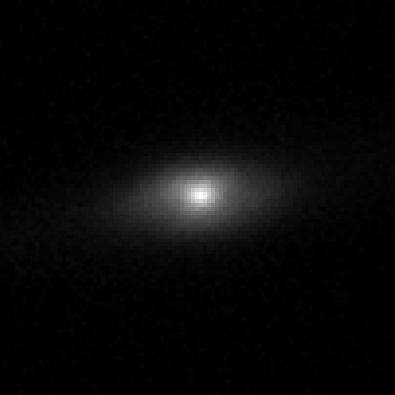
\includegraphics[scale=0.5]{big_galaxy.png}  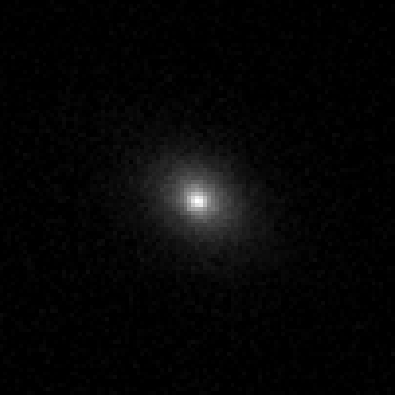
\includegraphics[scale=0.5]{inclined_galaxy.png}}
	\item Galaxy types: Galaxies are instrinsically of two types: spiral and elliptical. Examples are shown below. This can possibly play a role in constructing the PCA basis. In particular, spiral arms of spiral galaxies may be confused with rings themselves. \\ \\
	\end{itemize}
In conclusion, we need to standardize shapes, sizes and orientations of galaxy images in the sample.

\item Some properties of the photograph itself play a role, such as:
	\begin{itemize}
	\item Centering: If the object under consideration is off-center we have a problem: \\ \\
	\centerline{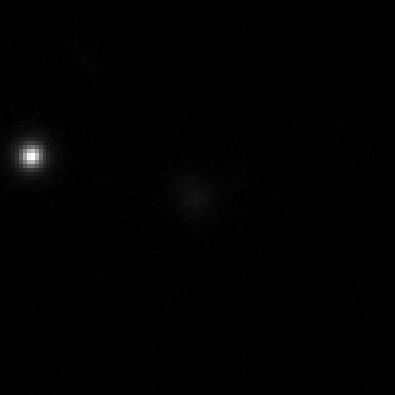
\includegraphics[scale=0.5]{non-centered_galaxy.png}} \\ \\
	\item Companions: Companions on galaxies are sources of artifacts. \\ \\
	\centerline{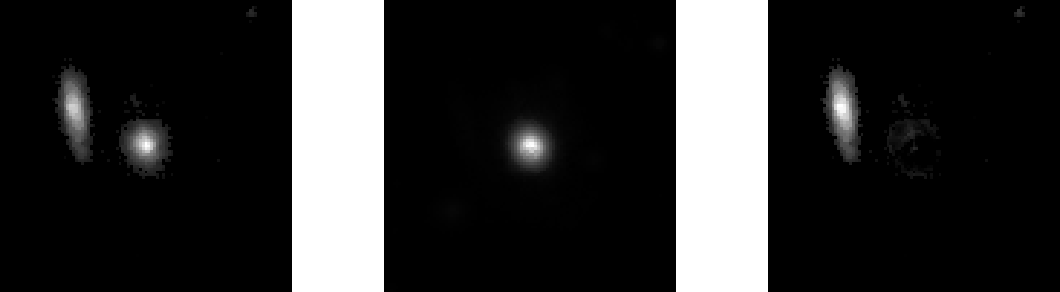
\includegraphics[scale=0.3]{1223_Source_Subtraction.png}}
	\\ \\ Here the left is the original, center is reconstructed and right is the residual image.
	\end{itemize}

\item Detector noise is very important, since most objects we image have noise of the order of the signal. So, we need to do significant denoising. \\ \\
\centerline{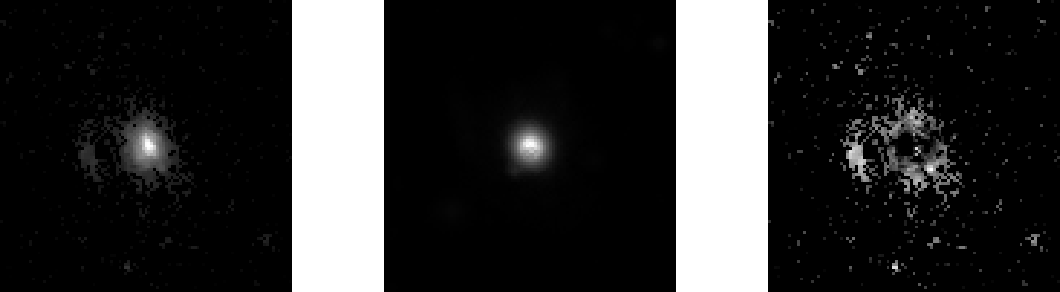
\includegraphics[scale=0.3]{1398_noise_amp.png}}
\end{itemize}

This leads to the next iteration. We have tried to correct some of the above issues here.

\subsection{Iteration 2}
We try to address the issue of sample sizes here. One simple way of handling sizes is to restrict data size itself to a certain radius. While acquiring images, a mask restricting the radius of the object was applied and then a basis was constructed. A median filter was applied to images before constructing the basis. While doing this has no theoretical reason, an approach like this can be used to weed out companions later. The first six of the 150 retained eigen-galaxies are shown below:\\ \\
\centerline{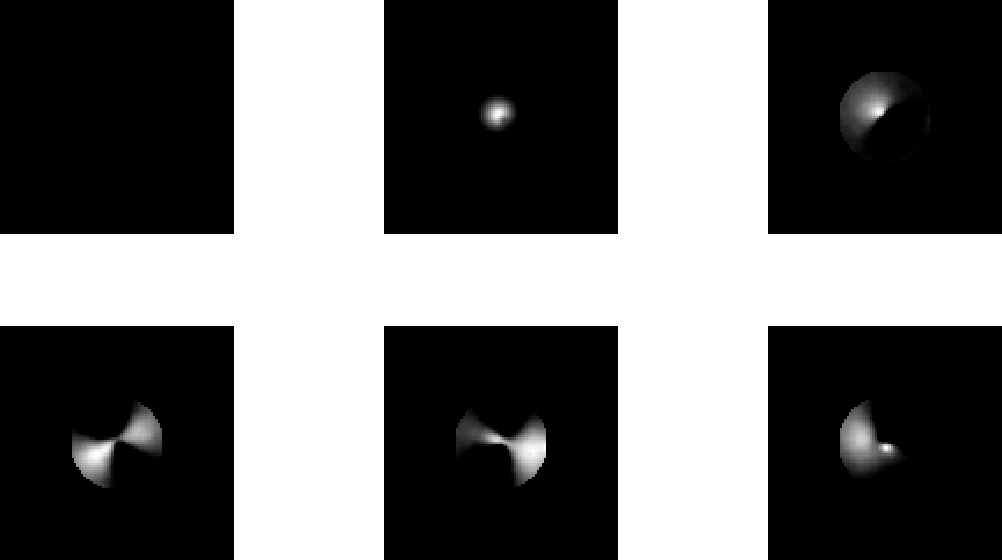
\includegraphics[scale=0.5]{aperture_limited_basis.png}} \\ \\
However this did not provide any good results for reconstruction of rings.

\section{Iteration 3}
Hence the only remaining option is to manually re-scale and re-align the sample so that all the spatial constraints are met. To test the method under such conditions, we selected $\sim$111 out of the 6000 galaxies whose centers were already aligned, had roughly same sizes and were not ambiguous with respect to existence of lenses. The eigen-galaxies here are shown below:\\ \\
\centerline{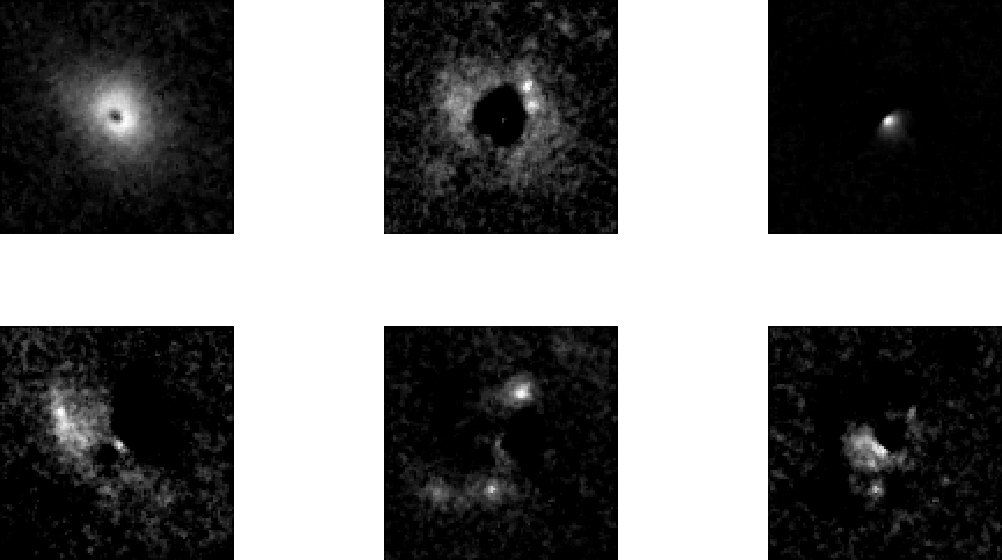
\includegraphics[scale=0.5]{limited_subset_basis.png}} \\ \\
We see here that the first four eigenvectors themselves are sufficient for reconstructing the central core of the lens. We included two eigenvectors in the reconstruction in this case. Below are some results, in the format original, reconstructed, residual.\\ \\
\centerline{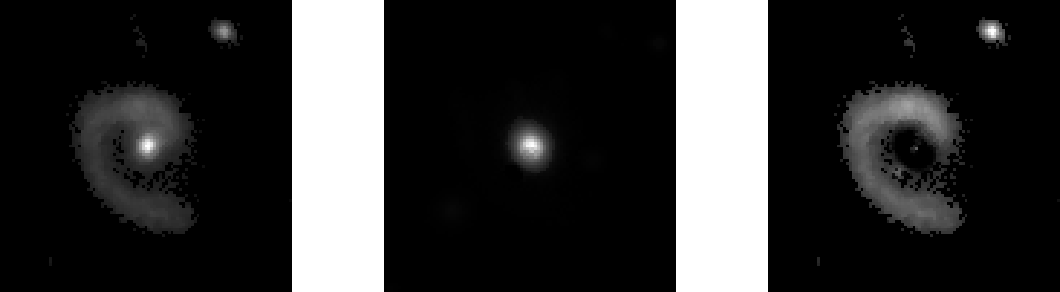
\includegraphics[scale=0.5]{4339_Final_Source_Subtraction.png}} \\ \\
\centerline{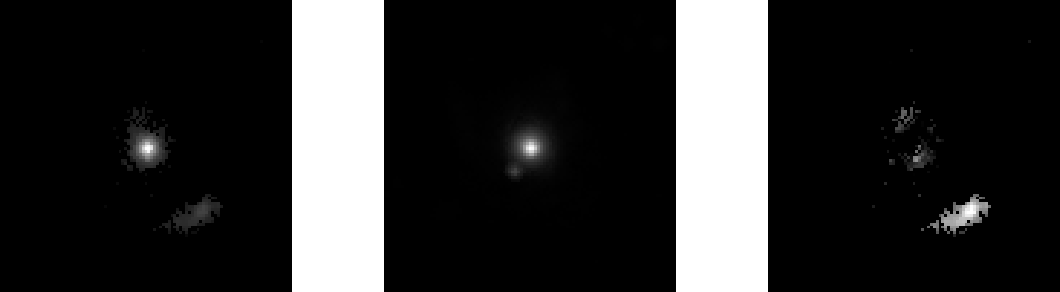
\includegraphics[scale=0.5]{704_Final_Source_Subtraction.png}} \\ \\
\centerline{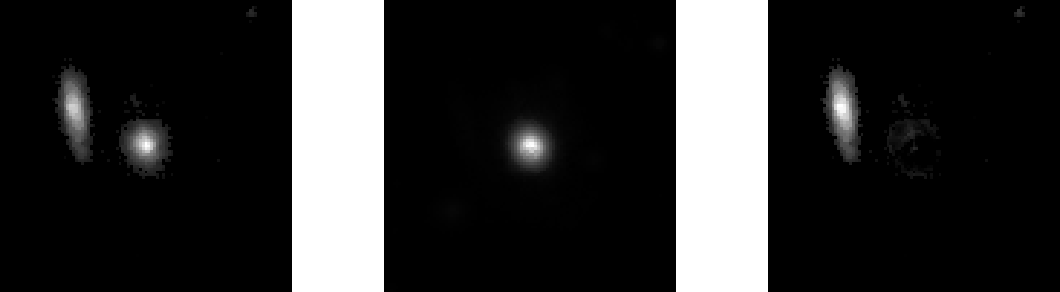
\includegraphics[scale=0.5]{1223_Source_Subtraction.png}} \\ \\
\centerline{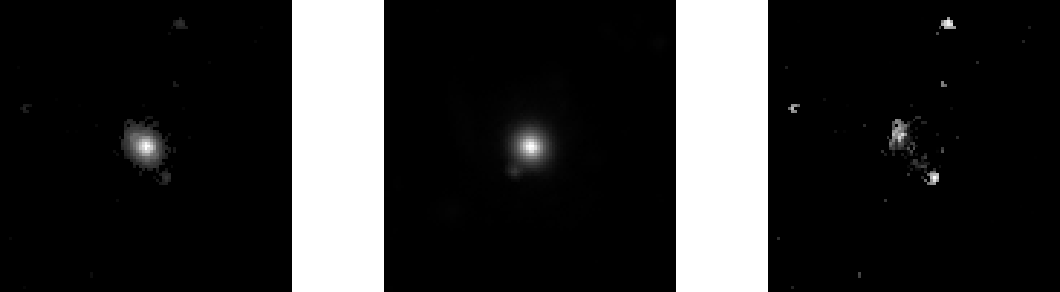
\includegraphics[scale=0.5]{1948_Source_Subtraction.png}} \\ \\
\centerline{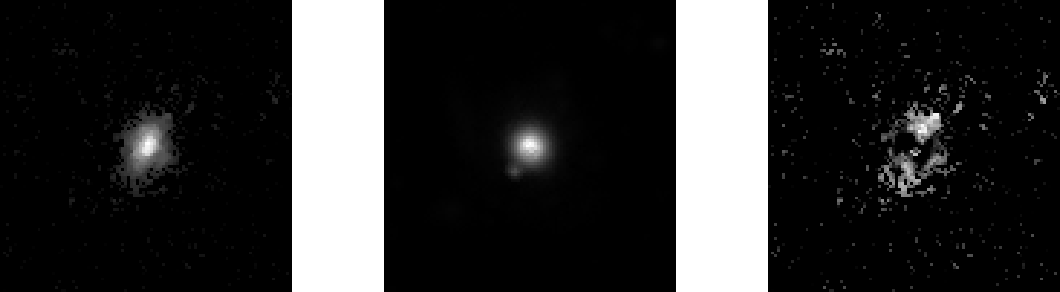
\includegraphics[scale=0.5]{3559_Final_Subtraction.png}} \\ \\
One example of a false positive (probably because of insufficiency of eigenvectors) is the following: \\ \\
\centerline{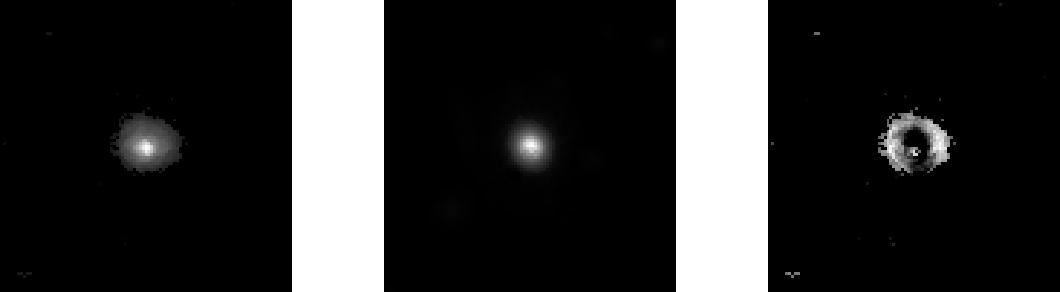
\includegraphics[scale=0.5]{1589_Failure_Case_False_Positive.png}} \\ \\
Among the 111 images taken here, 19 had lensing features and 3 were ambiguous spirals. Visually inspecting the output yielded 16 lenses whose rings were detected correctly and 6 false positives. Tuning the number of eigenvectors will resolve this problem.

\subsection{Corrections to be Applied in the Pipeline}
We will correct for the centering and scale here. Standard methods are also available for correcting rotations as well. \textit{Fill this up}

\subsection{Denoising}
\textit{Fill this up}

\subsection{Segmentation and Detection of Rings}
Once we do source subtraction we must segment the residual and check if we have a valid ring or not. The residuals we get may as well be reconstruction errors or noise.
The method we used for segmentation of residuals is the following: \textit{Fill this up}

\section{Conclusion}
Finding lenses in astronomical databases is an extremely non-trivial task, and in this project we have managed to scrape the easier lenses to find off. The problem of companions remains unsolved in our implementation. However, the idea is a good start to modelling galaxies on an observational level instead of traditional theoretical model-fitting approaches. A possible workaround to the companion problem and some areas to improve upon in this approach are suggested in the next section.
Lens parameter determination is an important problem because it is a good way of estimating the lensing galaxy's mass. Such mass estimates are of extreme importance in validating theories of galaxy evolution, structure formation and cosmology. With the volume of data expected to come in from surveys like CHFTLenS and others, it is justified to automate finding lenses and lens parameters.

\section{Future Scope and Problems With The Approach}
The companion problem is unresolved in out implementation. One possible workaround is presented here.

Once the residual from a source is segmented out, we need to identify if it is a galaxy or a lensed image. In general, lensed images of sources are very twisted and it would not be possible to reconstruct them using the PCA basis we constructed. On the other hand, in case of a companion we can easily reconstruct. So we reconstruct the segmented image using the basis and consider it a galaxy if the square error between the segmented and reconstructed images is smaller than a threshold. Otherwise, we consider it a lens.

Some work will have to be done on how to scale the galaxies themselves, because the scaling and rotation will invariably consider the lens itself. This will cause a problem in case the lens is bright.

Another addition would be to measure the arc parameters itself (arc angle, thickness and orientation with respect to the lens) once it is detected. This would involve a standard pattern-matching algorithm. This information can further be processed for mass determination or whatever other use.

Further problems and areas to work with would arise when further progress is made in this area.

\begin{thebibliography}{9}

\bibitem{joseph2014}
  R. Joseph, F. Courbin, \textit{et al.}
  \emph{A PCA-based Automated Finder for Galaxy-Scale Strong Lenses}.
  Astronomy \& Astrophysics
  2014.
  
\bibitem{matlab}
  The MATLAB Documentation at http://www.mathworks.in/help/matlab/

\end{thebibliography}

\end{document}